\documentclass[12px]{article}
\usepackage[cjk]{kotex}
\usepackage[top=2cm, bottom=4.5cm, left=2.5cm, right=2.5cm]{geometry}
\usepackage{amsmath, amssymb}
\usepackage{enumerate}
\usepackage{graphicx}

\title{응용통계학 4장 연습문제 풀이}
\author{20181653 이강희}
\date{}

\begin{document}
\maketitle

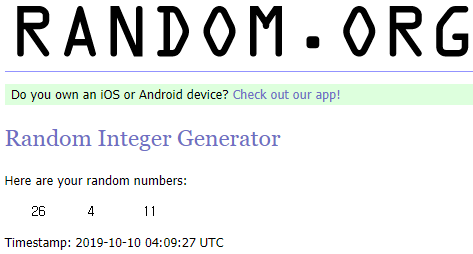
\includegraphics[scale=0.7]{random}

\section*{4번}
0점부터 시작해서 5점씩 20문제를 맞출 수 있다.\\
확률변수 X가 가질 수 있는 값은 0, 5, 10, ..., 100 이 있다.

\section*{11번}
\begin{enumerate}[(1)]
    \item
    \begin{flalign*}[t]
        P(X<4) &= \int_2^4 f(x) dx&\\
        &= \int_2^4 \frac{2(1+x)}{27} dx\\
        &= \left[\frac{2}{27}x + \frac{1}{27}x^2 \right]_2^4\\
        &= \frac{8}{27} + \frac{16}{27} - \left(\frac{4}{27} + \frac{4}{27}\right) = \frac{16}{27}
    \end{flalign*}
    \item
    \begin{align}
        P(X<4) &= \int_2^4 f(x) dx&\\
        &= \int_2^4 \frac{2(1+x)}{27} dx\\
        &= \left[\frac{2}{27}x + \frac{1}{27}x^2 \right]_2^4\\
        &= \frac{8}{27} + \frac{16}{27} - \left(\frac{4}{27} + \frac{4}{27}\right) = \frac{16}{27}
    \end{align}
\end{enumerate}

\section*{28번}
선수 중 왼손잡이의 비율이 35\% 이므로\\
임의로 한 선수를 선택했을 때 그 선수가 왼손잡이일 확률을 \(P(A) = 0.35 \) 라 한다.\\
오른손잡이일 확률은 \(P(A^C) = 0.65 \) 이다. (양손잡이는 고려하지 않음)
\begin{enumerate}[(1)]
    \item
    두 선수 모두 왼손잡이일 확률은 \(P(A) \times P(A) =  0.1225 \) 이다.
    \item
    한 선수는 왼손잡이, 한 선수는 오른손잡이일 확률은\\
    \(P(A) \times P(A^C) = 0.35 \times 0.65 = 0.2275 \) 이다.
    \item
    적어도 한 선수는 오른손잡이일 확률은 모두 왼손잡이일 확률의 여집합이므로\\
    \(1 - P(A) \times P(A) = 1 - 0.1225 = 0.8775 \) 이다.
\end{enumerate}

\end{document}